\documentclass[a4paper,twoside]{article}

%% Language and font encodings
\usepackage[spanish]{babel}
\usepackage[utf8]{inputenc}
\usepackage[T1]{fontenc}


%% Sets page size and margins
\usepackage[a4paper,top=3cm,bottom=2cm,left=2.5cm,right=2.5cm,marginparwidth=0.5cm]{geometry}

\usepackage{amsmath}			%Paquete matemático
\usepackage{graphicx}
\usepackage[colorinlistoftodos]{todonotes}

\usepackage{hyperref}		%Paquete empleado para colocar hipervinculos
\hypersetup{
	colorlinks = true,
	linkcolor = black,
}

\usepackage{eurosym}
\usepackage{pdfpages}			%Sirve para incluir PDF en el documento
\usepackage{anysize}			%Podremos colocar imagenes de cualquier tamaño
\usepackage{subfig}				%Nos permitira colocar varias imagenes en una figura
\usepackage{float}				%Podremos crear y colocar boxes donee queramos
\usepackage[export]{adjustbox}

%Colocamos cabeceras y pies de pagina
%(CONSULTA: http://edicionesoniricas.com/maquetar-latex-encabezados-pies-pagina/)
%(CONSULTA2: https://es.sharelatex.com/learn/Headers_and_footers)
%\bfseries es análogo a \textbf{}
% \leftmark-> Adds name and number of the current top-level structure (section for article) in uppercase letters.
%\rightmark-> Adds name and number of the current next to top-level structure (subsection for article) in uppercase letters.
\usepackage{fancyhdr}		%Paquetes necesarios
\pagestyle{fancy}			%Borra los parametros por defecto
\fancyhf{}
\fancyhead[RO,LE]{\bfseries\thepage}
\fancyhead[LO,RE]{\bfseries\rightmark}
%Nos aseguramos de que en las paginas plain, no haya ni cabeceras ni lineas
\fancypagestyle{plain}
{
	\fancyhead{} % elimina cabeceras en paginas "plain"
	\renewcommand{\headrulewidth}{0pt} % así como la raya
}

%Definimos las lineas divisoras de las cabeceras y pie de pagina
\renewcommand{\headrulewidth}{1pt}	%Define el grosor de la línea de head
\renewcommand{\footrulewidth}{0pt}		%Define el grosor de la linea foot (Si no queremos linea, 0pt)
\addtolength{\headheight}{0.5pt} % espacio para la raya

%Librerias para introducir código de Matlab
%\usepackage{bigfoot} % to allow verbatim in footnote
\usepackage[numbered,framed]{matlab-prettifier}
\usepackage{listings,lstautogobble}
\lstset{
	style              = Matlab-editor,
	basicstyle         = \mlttfamily,
	escapechar         = ",
	mlshowsectionrules = true,
	autogobble=true
	language=Matlab
}

% Pie de pagina
%\fancyfoot{} % limpia el pie
\fancyfoot[C]{- \thepage -} % número de página centrado

%Nos generará texto para pruebas de maquetado
\usepackage{lipsum}

% Se varia el limite de colimnas de latex
\setcounter{MaxMatrixCols}{11}
\usepackage{lscape}
%----------------------------------------------------------------------------------------------------------------------------------
\begin{document}
\begin{titlepage}
	\centering
\Huge{\textbf{CONTROL Y PROGRAMACIÓN DE ROBOTS}} \\
\Huge{\textit{Proyecto de robótica móvil}}\\

\vspace{1cm}
\LARGE{Grado en Ingeniería Electrónica, Mecatrónica y Robótica}\\
\rule{\textwidth}{0.1mm}
%  %%%%% Este trozo de codigo es para insertar imagenes %%%%%%%
\begin{figure}[h!]
	\centering
	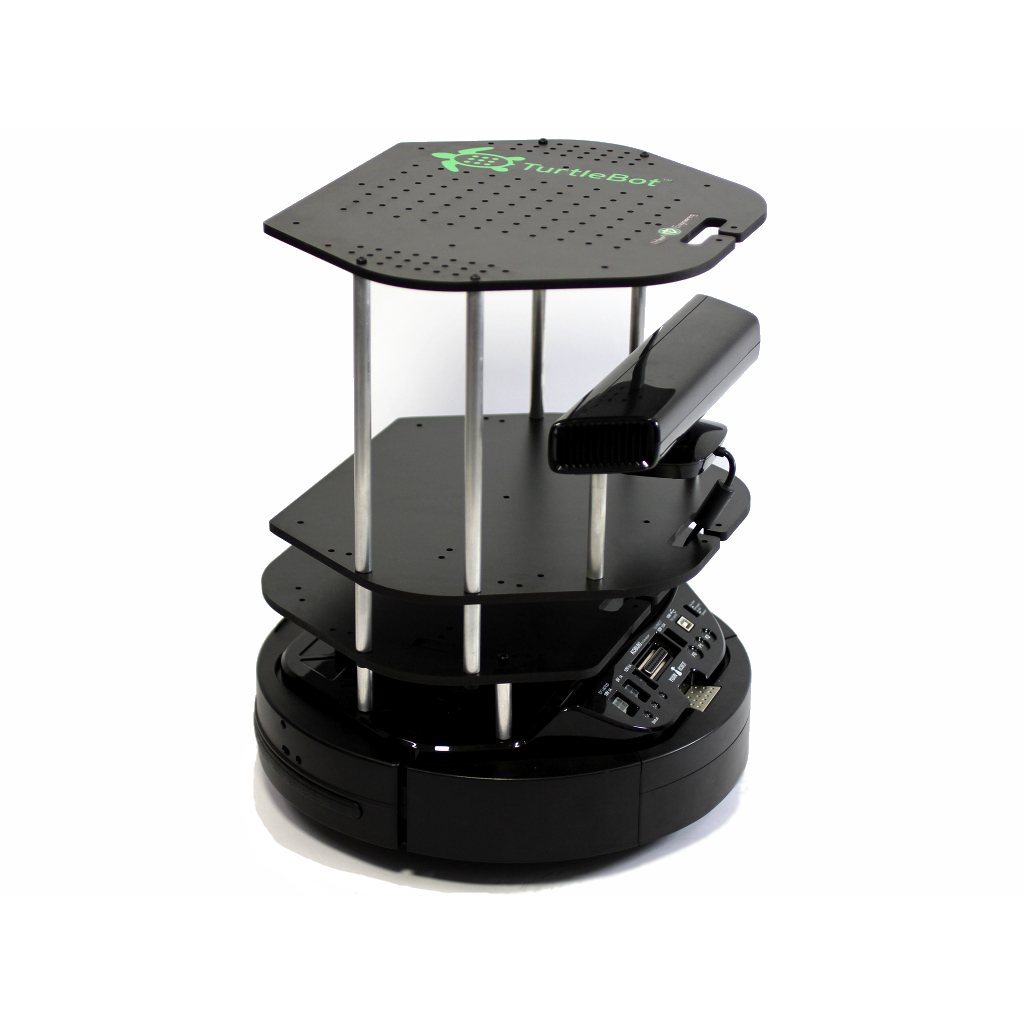
\includegraphics[width=.7\textwidth]{robot_portada}
	%\caption{textodelaleyenda}
\end{figure}
% %%%%%%%%%%%%%%%%%%%%%%%%%%%%%%%%%%%%%%%%%%%%%%%%%%%%%%%%%%%%%
\vspace{1cm}
\rule{\textwidth}{0.1mm}
\Large{\textbf{Autores:} Montes Grova, Marco Antonio\\
 Lozano Romero, Daniel\\
 Mérida Floriano, Javier}
\end{titlepage}
\tableofcontents
\newpage
% %%%%%%%%%%%   INTRODUCCION %%%%%%%%%%%%%%%%%%
\section{Introducción al proyecto}
En el proyecto que sigue a continuación se desarrollará el modelado y control de un robot móvil tipo síncrono. La principal característica destacable de este tipo de robots recae en el mecanismo mecánico interno que posee mediante el cuál se podrán mover 3 ruedas empleando únicamente 2 motores.\\
Con uno de los motores se desplazará en línea recta y con el otro se le dará el ángulo de giro deseado sobre sí mismo.\\

El modelo síncrono se basa en 3 ruedas idénticas que se desplazan y giran al unísono, haciendo posible que el robot pueda moverse en cualquier dirección y orientación en el plano del suelo. Estas ruedas están dispuestas de forma triangular en la base del robot, el cual se va a representar como un objeto cilíndrico, siendo la base uno de los lados circulares. Par un mayor entendimiento, se va a representar un esquema del mecanismo utilizado en este tipo de robot móvil:\\

\begin{figure}[h!]
	\centering
	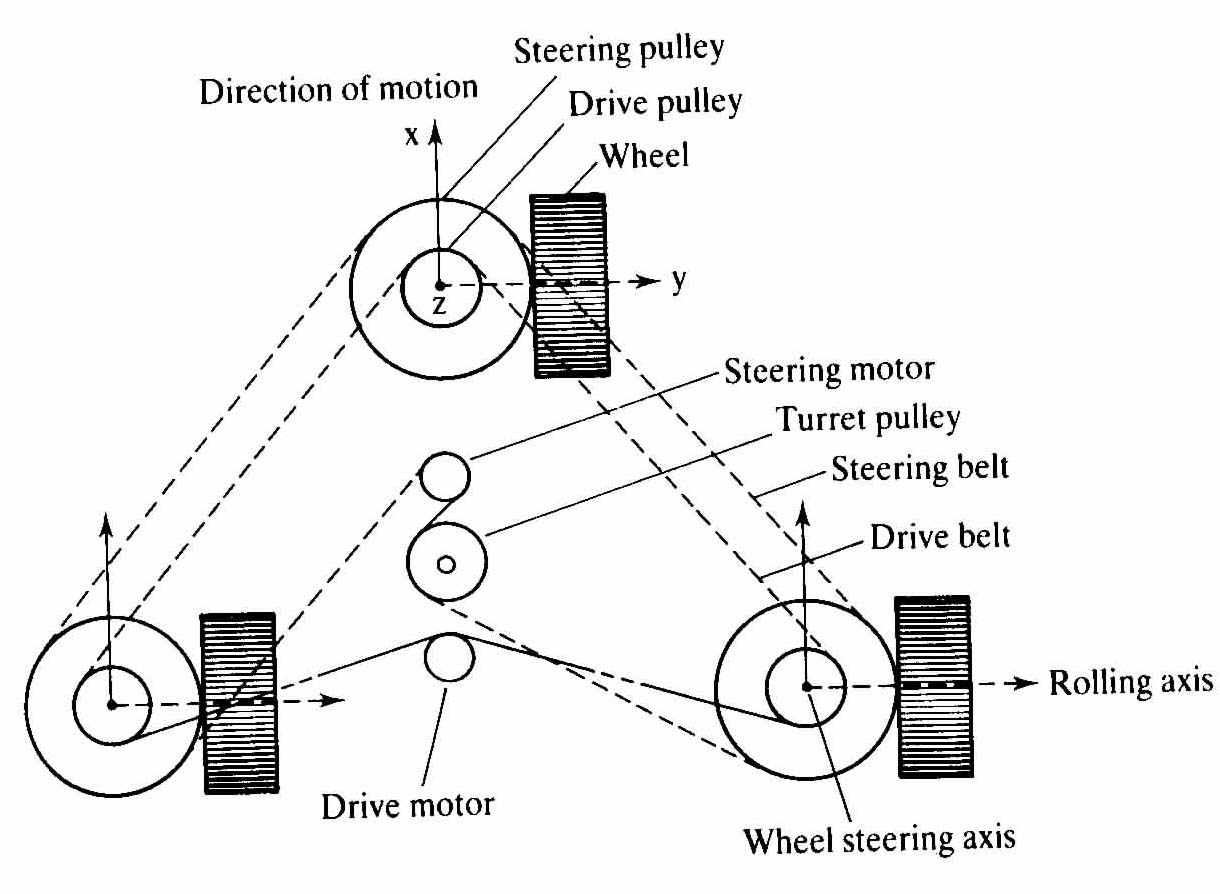
\includegraphics[width=.6\textwidth]{mecanismo_interno}
\end{figure}

Este modelo tiene como ventajas la separación de motores entre traslación y rotación que facilita el control, la garantía de control en trayectorias rectilíneas debido a la mecánica del mismo y la facilidad que incluyen las restricciones homólogas que posee. Como desventaja encontramos el complejo diseño mecánico que posee para poder transmitir la rotación y traslación a las tres ruedas simultáneamente y, por ende, su difícil implementación en la realidad.\\
% SEGUIR HABLANDO DE MOVIDAS TEORICAS UN PSEUDO LARGO TRECHO ETC ETC ETC ETC

\section{Análisis cinemático}
	\subsection{Introducción teórica y simplificación del modelo}
	Gracias a la mecánica del modelo síncrono, los cálculos para la obtención del modelo cinemático del mismo van a ser sencillos, ya que se trata de un modelo con restricciones holónomas, es decir, el comportamiento del vehículo se puede representar a través de sus variables generalizadas:
	\begin{itemize}
		\item Las variables cartesianas \textit{X} y \textit{Y} como coordenadas del centro del robot en el plano del suelo.
		\item La variable angular $\varphi$ como la rotación producida frente al estado inicial, es decir, cuando éste vale cero.
	\end{itemize}
	las cuales son integrables en el tiempo de tal modo que resulta sencillo la obtención de un modelo cinemático de posiciones y velocidades.\\
	La postura del robot, se podría obtener a partir de la aplicación de una matriz de rotación en torno al eje perpendicular al plano de suelo, es decir, respecto al eje Z:
	\begin{equation}
		R(\varphi)=
		\begin{bmatrix}
			cos\varphi & sin\varphi & 0 \\
			-sin\varphi & cos\varphi & 0 \\
			0 & 0 & 1
		\end{bmatrix}
	\end{equation}
	Además de ello, cabe destacar que, para simplificar el modelado del robot, se han asumido una serie de restricciones cinemáticas en las ruedas cómo son:
	\begin{itemize}
		\item Movimiento en un plano horizontal.
		\item Las ruedas poseen un único punto de contacto.
		\item Las ruedas no son deformables.
		\item $v_c$ en el punto de contacto será nulo.
		\item La rueda no resbala, sino que produce un movimiento de arraste o deslizamiento.
		\item No habrá fricción en el punto de contecto.
		\item Los ejes de dirección serán en todo momento ortogonales a la superficie.
		\item Las ruedas están conectadas al bastidor de giro.
	\end{itemize}

\subsection{Obtención del modelo cinemático directo y su Jacobiano}
Para el modelo cinemático directo en cuestión, sólo se necesita como dato el valor del radio de las ruedas, $R$, para poder realizar la conversión entre velocidad angular y velocidad lineal. En este trabajo, siendo el grupo de trabajo número 11, se tiene cómo radio de las ruedas el valor de $R = 0.4 m$. Con esto ya se puede hallar el modelo cinemático del robot:\\

	Para comenzar se deben definir las variables generalizadas y de actuación del sistema, respectivamente:
	\begin{center}
		$
		q=
		\begin{bmatrix}
		x\\
		y\\
		\varphi
		\end{bmatrix}
		$$
		\hspace{2cm}
		$$
		p=
		\begin{bmatrix}
		\dot{\theta} \\
		\omega
		\end{bmatrix}
		$
\end{center}

Como ya vio en las clases de la asignatura, las variables generalizadas son las que dan información sobre el estado del robot, ya que se encuentran en ellas las coordenadas cartesianas \textit{X} e \textit{Y} del plano del centro del robot y el ángulo de giro $\varphi$ con respecto al eje X, como se ha decidido definir en este proyecto.\\
Así mismo, las variables de actuación son, como dice su nombre, las variables que reflejarán el valor de movimiento de los motores del robot, es decir, del motor encargado del desplazamiento (velocidad lineal, $\dot{\theta}$) y del encargado de la rotación (Velocidad angular, $\omega$).\\

Una vez detectadas las variables del sistema, se deberá definir la relación entre ellas y, de ese modo,obtener la expresión del Jacobiano, es decir, la relación entre la derivada de las variables articulares de salida y de entrada.\\
En primer lugar, se definirá $v$ como la componente global de velocidad de desplazamiento, por tanto, se calculará como:
\begin{center}
	$v^2=\dot{x}^2+\dot{y}^2$ o como $v=R \dot{\theta}$
	\end{center}
	y, a su vez, la componentes cartesianas de la velocidad se definirán como:
	\begin{center}
	$\dot{x}=v cos(\varphi)$\\
	$\dot{y}=v sin(\varphi)$
	\end{center}


	Sabiendo además que la velocidad de rotación $\dot{\varphi}$ concuerda con la variable de actuación $\omega$, se puede montar la matriz Jacobiana del sistema del mismo que se dijo anteriormmente, es decir:
\begin{center}
		$
		J=
		\begin{bmatrix}
			R cos(\varphi) && 0\\
			R sin(\varphi) && 0\\
			0 && 1
		\end{bmatrix}
		$
\end{center}

La matriz Jacobiana describirá la cinemática directa del sistema relacionando las variables de actuación con las derivadas de las variables generalizadas y, como se sabe que serán integrables debido a la existencia de restricciones holónomas, se podrán integrar para poder hallar los valores de posición y orientación.\\

	Dicho esto, se puede expresar el modelo cinemático como función de entradas (variables de actuación) y salidas (variables generalizadas):
	\begin{equation}
		\begin{bmatrix}
		\dot{x}\\
		\dot{y}\\
		\dot{\varphi}
		\end{bmatrix}
		=
		\begin{bmatrix}
		R cos(\varphi) && 0\\
		R sin(\varphi) && 0\\
		0 && 1
		\end{bmatrix}
		\begin{bmatrix}
		\dot{\theta}\\
		\omega
		\end{bmatrix}
	\end{equation}

	e integrando respecto del tiempo éstas matrice,se obtendrá:
		\begin{equation}
		\begin{bmatrix}
		x\\
		y\\
		\varphi
		\end{bmatrix}
		=
		\begin{bmatrix}
		x_0\\
		y_0\\
		\varphi_0
		\end{bmatrix}
		+
		\begin{bmatrix}
		\int_{0}^{t} R\dot{\theta}cos(\varphi)dt\\
		\int_{0}^{t} R\dot{\theta}sin(\varphi)dt\\
		\int_{0}^{t} \omega dt
		\end{bmatrix}
	\end{equation}

	dónde $x_0$, $y_0$ y $\varphi_0$ serán las condiciones iniciales de posición y orientación.\\
	\subsubsection{Esquema de simulación del modelo directo obtenido}
	Una vez obtenido el modelo cinemático directo se implementará en una función en Matlab, la cuál servida para modelar el comportamiento del movimiento del robot. Por tanto, el modelo cinematico directo se implementará del siguiente modo:
	% AQUI VA EL CODIGO DE PRUEBAS MCD -> METIDO EN UN ANEXO
	\lstinputlisting[caption = {Implementación del modelo cinemático directo}]{MCD_movil.m}

	A continuación, se mostrará el montaje completo en Simulink que ha sido utilizado para obtener los resultados de la simulación.
	\begin{figure}[h!]
		\centering
		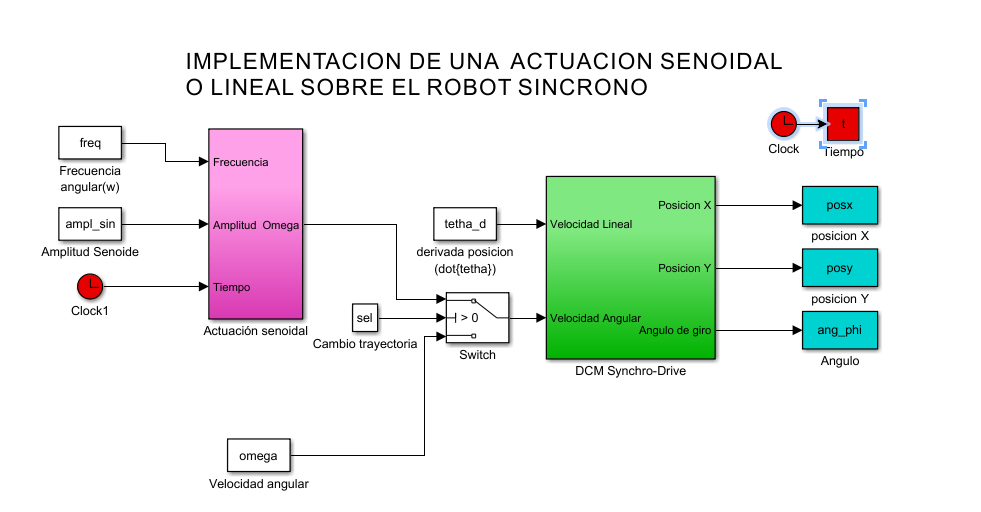
\includegraphics[width=.8\textwidth]{simulink_MCD_1}
		\caption{Esquema global}
	\end{figure}

En éste montaje existen dos subsistemas, los cuales se mostrarán a continuación. El primero de ellos, será el encargado de generar una actuación senoidal sobre el sobor, de tal modo que siga una trayectoria de éste tipo.
\begin{figure}[h!]
	\centering
	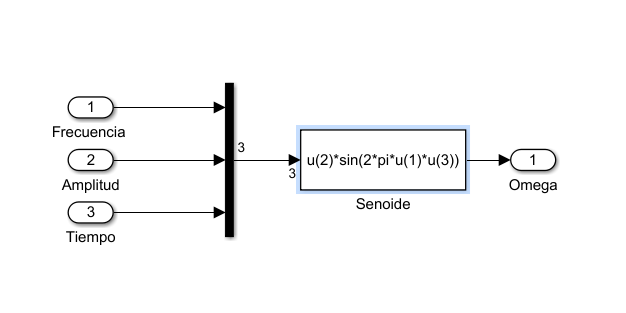
\includegraphics[width=.5\textwidth]{simulink_MCD_2}
	\caption{Esquema del bloque \textit{Actuación Senoidal}}
\end{figure}

 El segundo de ellos, será la implmentación del modelo cinemático directo del robot en un bloque, en el cuál se relamientará la variable angular, la cual es una variable de entrada y de salida del modelo y, además de ello, se saturarán las actuaciones.
 \begin{figure}[h!]
	 \centering
	 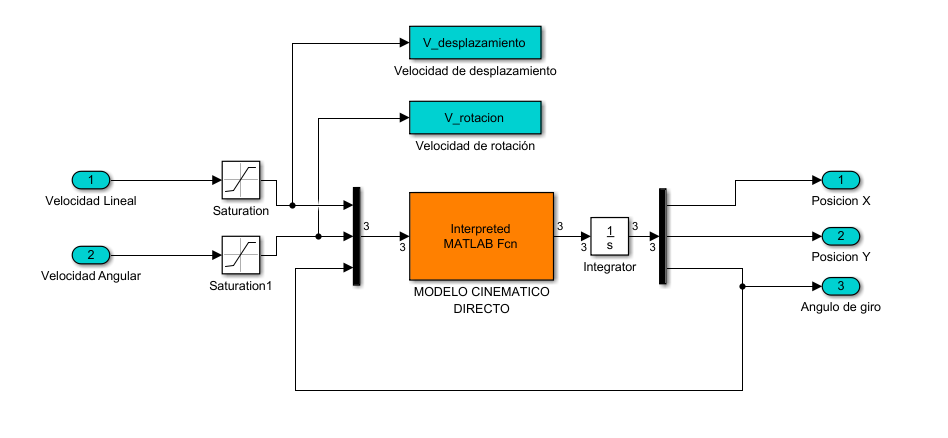
\includegraphics[width=.65\textwidth]{simulink_MCD_3}
	 \caption{Esquema del bloque \textit{DCM Synchro-Drive}}
 \end{figure}

\newpage
Cabe destacar cómo se saturarán las variables del modelo; la velocidad angular, se limitará a aproximadamente $\pm$ 15 grados por segundo, ya que es el angulo máximo aproximado al que teóricamente se puede girar un volante. En cuando a la velocidad lineal, se limitará aproximadamente a 30 centímetros por segundo, que correspondería aproximadamente a 1 km/h, lo cuál se considera una velocidad suficiente para un robot móvil.\\

Antes de introducir los experimentos realizados, cabe destacar que en un anexo se encontrarán los códigos de programación implementados para realizar dichos experimentos.

\subsubsection{Experimentos realizados al modelo para su verificación}
Con este código se pueden realizar varios experimentos. Para todos ellos las características comunes serán que partirán de las mismas condiciones iniciales para las variables generalizadas ($x=0, y=0, \varphi=0$) y tendrán las mismas saturaciones, las cuales hemos supuesto como realistas para este tipo de robot.\\
	\begin{itemize}

		\item \textbf{Primer experimento} \\
	El primer experimento que se va a mostrar es el de una velocidad de desplazamiento máxima y velocidad de rotación nula. Como la simulación dura 30 segundos, el robot deberá recorrer una distancia de 9 metros:

	\begin{figure}[h!]
		\centering
		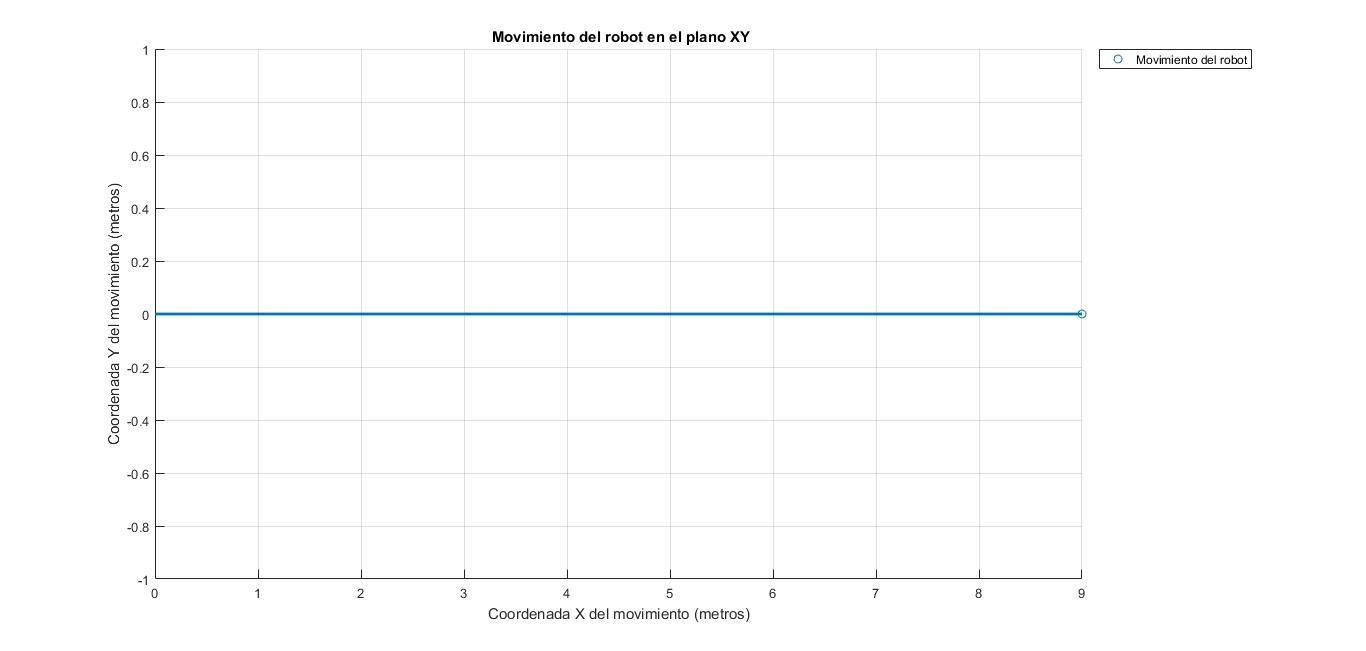
\includegraphics[width=1\textwidth]{exp_MCD_1}
		\caption{Movimiento en el plano con actuación de desplazamiento constante y rotativa nula}
	\end{figure}

\newpage
	\item \textbf{Segundo experimento} \\
	El siguiente experimento combinará ambas variables de actuación, estableciendo el valor máximo en ambas, por lo que el robot deberá dar vueltas en círculo. Como la velocidad de rotación máxima es de 15 grados/segundo y la simulación dura 30 segundos, el robot deberá dar 1 vuelta y 1/4 de vuelta más. En este y el siguiente experimento, al no constar únicamente de una trayectoria rectilínea, se ha aprovechado para representar, a través de flechas, el vector velocidad de desplazamiento:

	\begin{figure}[h!]
		\centering
		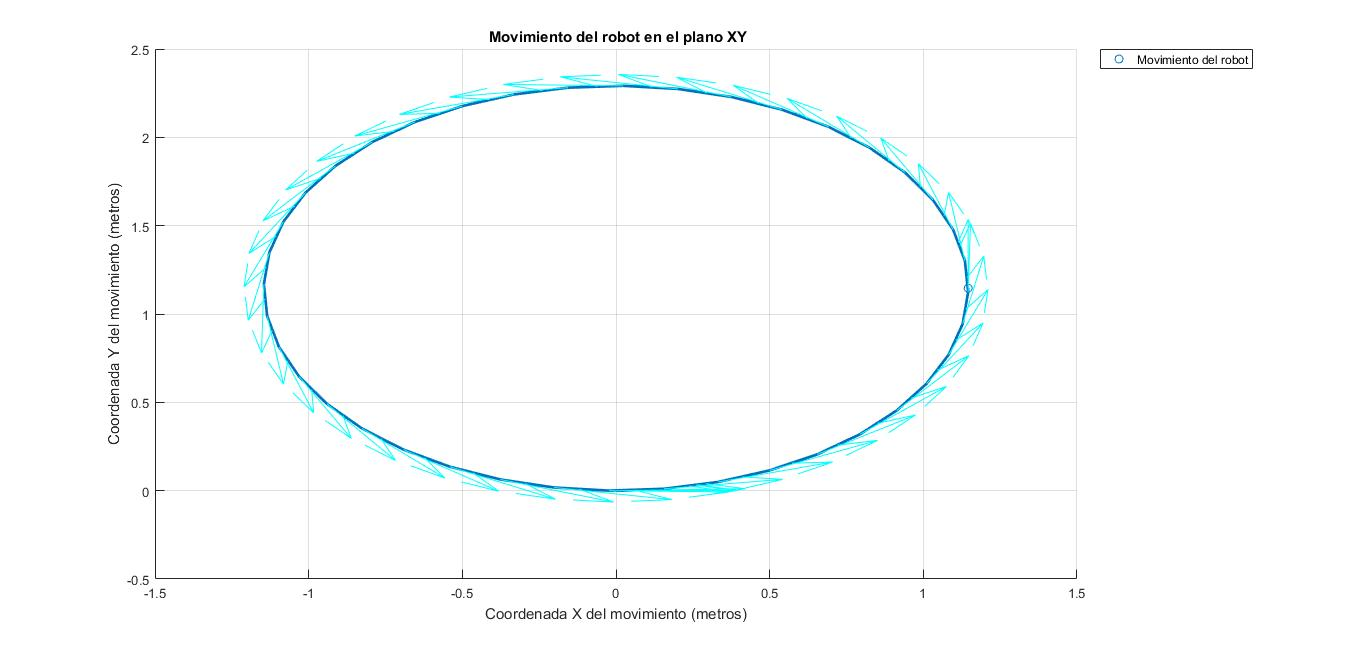
\includegraphics[width=1\textwidth]{exp_MCD_2}
		\caption{Movimiento en el plano con actuación de desplazamiento y rotativa constantes}
	\end{figure}

	\item \textbf{Tercer experimento} \\
	Ahora se va a realizar el experimento correspondiente a la prueba solicitada para el trabajo donde se ha de administrar una velocidad de desplazamiento constante y una velocidad de rotación con carácter senoidal. Para ello, se ha introducido una velocidad de desplazamiento de 0.5 radianes/segundo y una senoide de 0.05 Hz de frecuencia y 0.2 radianes/segundo de amplitud:
	\begin{figure}[h!]
		\centering
		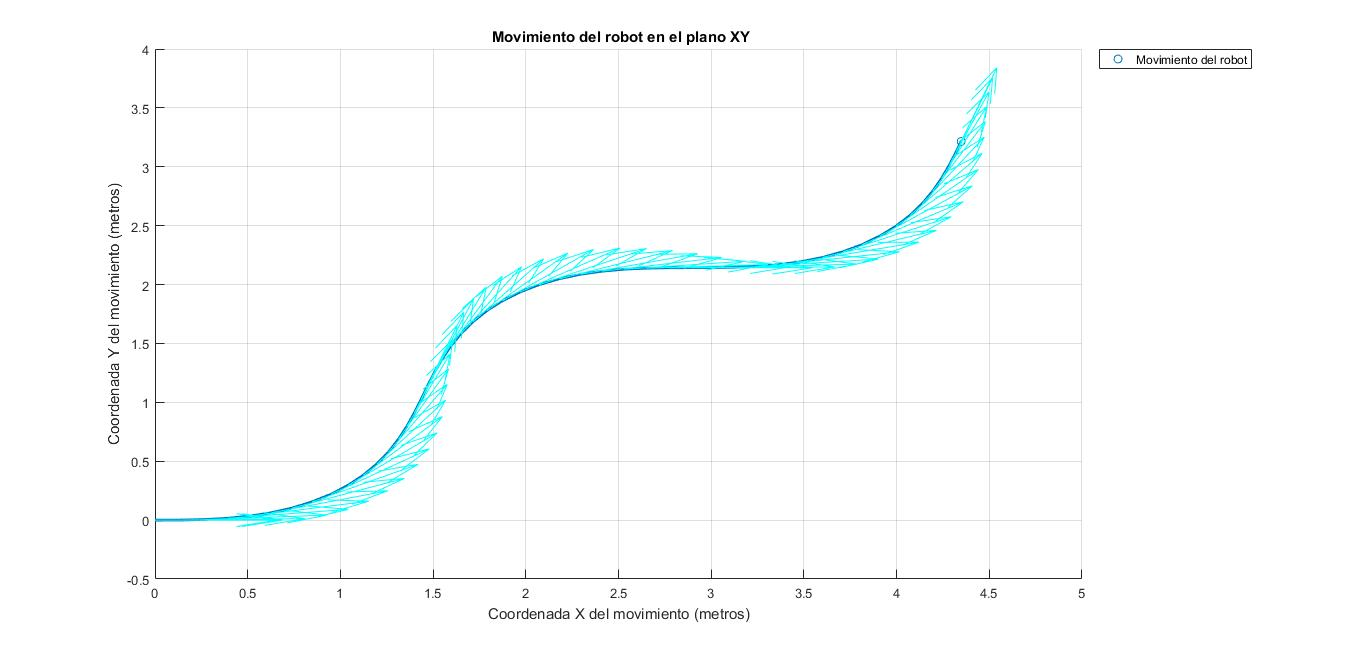
\includegraphics[width=1\textwidth]{exp_MCD_3_1}
		\caption{Movimiento en el plano con actuación rotativa senoidal}
		\label{exp_MCD_3_1}
	\end{figure}

	En este último experimento se puede observar que la variable de actuación $\omega$ resulta la senoide esperada y que, como resultado, se obtiene también una trayectoria senoidal, cómo se observa en la figura número \ref{exp_MCD_3_1}.\\

	\begin{figure}[h!]
		\centering
		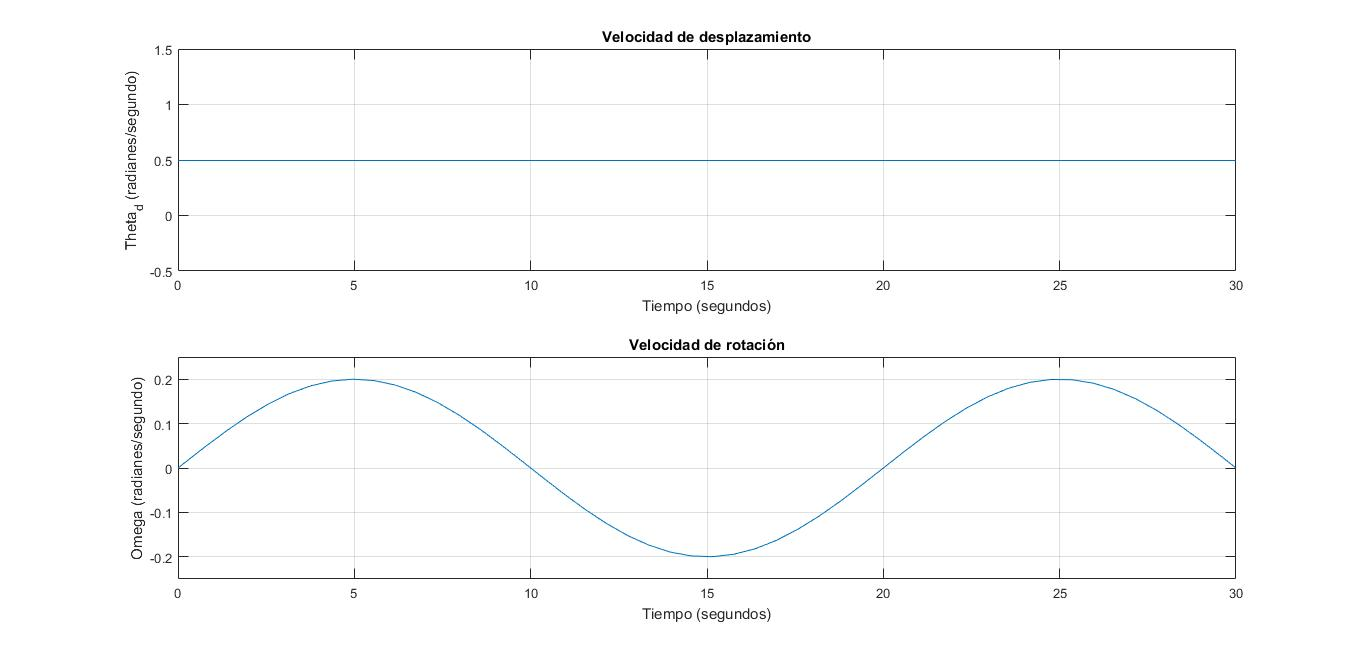
\includegraphics[width=1\textwidth]{exp_MCD_3_2}
		\caption{Variables de actuación tras saturación (arriba $\dot{\theta}$ y abajo $\omega$)}
		\label{exp_MCD_3_2}
	\end{figure}
	\end{itemize}

\newpage
	\subsection{Obtención del modelo cinemático inverso}
Una vez comentado todo lo que concierne a la cinemática directa, se puede pasar a obtener el modelo cinemático inverso, el cual será de utilidad para la creación de trayectorias con las variables generalizadas y su posterior transformación a variables de actuación que harán que el robot siga dicha trayectoria.\\

Dicho esto, el modelo cinemático inverso se basa principalmente en la Jacobiana inversa, ya que ahora se desea relacionar las variables generalizadas como entradas con las variables de actuación como salida. Por ello únicamente hay que coger la ecuación del modelo cinemático directo y pasar el Jacobiano al otro lado, es decir, poner su inversa. \\

En este caso se da que el Jacobiano del modelo directo no es una matriz cuadrada, por lo que no puede tener inversa, así que habrá que realizar la pseudoinversa del mismo. Para ello, no es necesario realizar los cálculos paso por paso, ya que MATLAB posee una función que calcula la pseudoinversa por el método Moore-Penrose llamada $pinv$. Dicho esto, una vez utilizada la función y habiendo simplificado, el resultado es:
\begin{equation}
	J^{-1}=
	\begin{bmatrix}
	\dfrac{cos(\varphi)}{R} && \dfrac{sin(\varphi)}{R} && 0\\
	0 && 0 && 1
	\end{bmatrix}
\end{equation}


Una vez obtenida la expresión del Jacobiano inverso, simplemente bastaría con introducirle los datos de entrada necesarios ($\dot{x}$, $\dot{y}$ y $\dot{\varphi}$) para obtener las salidas esperadas ($\dot{\theta}$ y $\omega$).\\

Para garantizar el funcionamiento del modelo inverso, se va a realizar el tercer apartado del proyecto, donde se pide obtener las señales de control necesarias para que el robot realice una trayectoria parabólica, la cual va a venir dada por la expresión:

\begin{center}
 $y=-\dfrac{x(x-A)}{D}$
\end{center}
donde, \textit{X} e \textit{Y} son las coordenadas cartesianas de la posición del centro del robot, $A$ una constante que determinará el valor máximo en $x$ que alcanzará la parábola y $D$ otra constante que determinará el valor máximo en $y$ que alcanzará la parábola.\\

	\subsubsection{Esquema de simulación del modelo inverso obtenido}
Para explicar como se ha llevado a cabo el proceso de obtención de los resultados, se va a hacer uso del montaje en Simulink utilizado en esta parte:
\begin{figure}[h!]
	\centering
	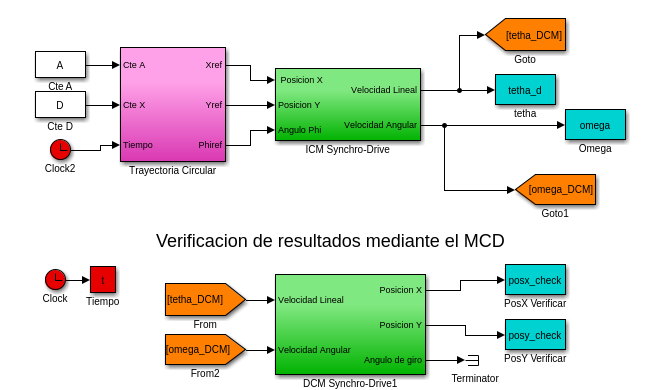
\includegraphics[width=.7\textwidth]{simulink_MCI_1}
	\caption{Esquema global}
\end{figure}

%Dado el esquema global utilizado para la simulación del experimento, se va a empezar a explicar en orden de ejecución, por lo que se %comenzará por el bloque de "Trayectoria Parabólica":

%\begin{figure}[h!]
%	\centering
%	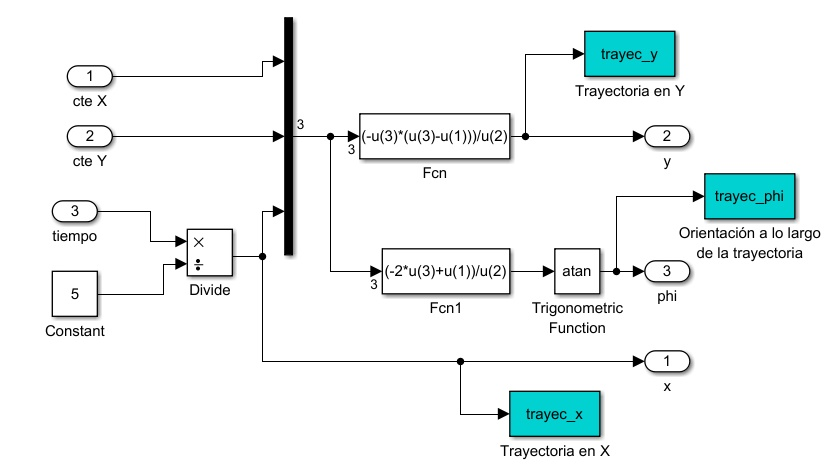
\includegraphics[width=1\textwidth]{simulink_MCI_2}
%	\caption{Bloque de Trayectoria Parabólica}
%\end{figure}

Como se pudo observar, las entradas a este bloque son las 2 constantes (\textit{A} y \textit{D}) de la parábola y el tiempo de simulación. Las dos primeras son utilizadas para la formulación de la parábola en sí y la tercera para la definición de \textit{X} que crecerá linealmente pero a una escala 5 veces más pequeña que el tiempo de simulación.\\

Para trazar la trayectoria se ha implementado la siguiente función en matlab, la cuál se implementará en Simulink cómo de costumbre. La salidas de dicha función serán las que se ven en el esquema de Simulink mostrado anteriormente.

\lstinputlisting[caption = {Implementación trayectoria parabolica}]{tray_parab.m}


%A la derecha del multiplexor se encuentra una primera función que determinará el valor de \textit{Y}, es decir, es la función de la %parábola, tal y como se había descrito anteriormente.\\
%Un poco más abajo se encuentra otra función que en realidad la derivada de la primera, puesto que se busca calcular la tangente a la %parábola en cada instante para así poder obtener la pendiente de dicha recta, realizar la arcotangente y hallar el ángulo que conforma %con el eje X, que coincidirá con la definición del ángulo $\varphi$.\\

Una vez se han definido los puntos de la trayectoria que ha de seguir el robot y con qué orientación ha de hacerlo, simplemente hay que pasar dichos datos al bloque donde se encuentra el modelo cinemático inverso:

\begin{figure}[h!]
	\centering
	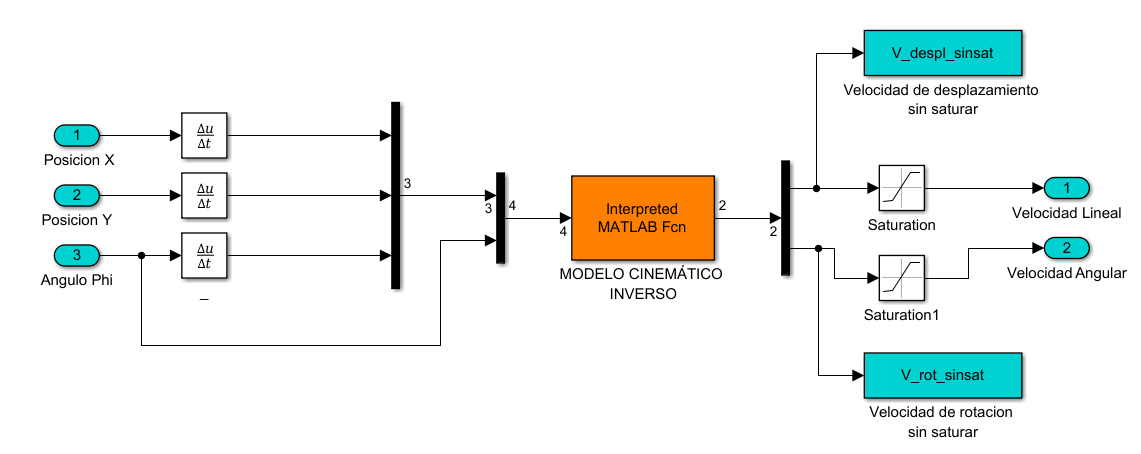
\includegraphics[width=.7\textwidth]{simulink_MCI_3}
	\caption{Bloque dónde se implementa la cinemática inversa del robot}
\end{figure}

Como se puede observar, lo primero que se debe hacer es derivar cada una de las entradas respecto al tiempo, puesto que el Jacobiano inverso, como antes lo hacía el directo, considera relaciones entre velocidades. Cabe destacar que, derivar computacionalmente no es una buena técnica, debido a que añade una componente elevada de error, sin embargo, en éste caso, dicha componente es asumible. Si en alguna otra ocasión fuese posible, sería mucho mas conveniente integrar una velocidad para conocer la posición que derivar una posición para conocer la velocidad.\\

\newpage
Una vez hecho eso, se introducen los valores en el bloque que contiene a la función que ejecuta la cinemática inversa, cuyo código se muestra a continuación:

\lstinputlisting[caption = {Modelo cinemático inverso del robot sincrono}]{MCI_movil.m}

Se observa que simplemente se realiza la multiplicación matricial para obtener las variables de actuación.\\

Por último, antes de volver al esquema global, se saturan los valores de estas salidas con las mismas saturaciones que se habían determinado realistas en la cinemática directa.\\
Para terminar, en el esquema global, se coloca de nuevo el bloque de la cinemática directa para comprobar, con las variables de actuación obtenidas con el modelo inverso, se obtiene la misma trayectoria que se ha diseñado.\\

\newpage
\subsubsection{Experimentos realizados al modelo inverso para su verificación}
Con el montaje en Simulink ya creado, lo único que falta es lanzar un script que asigne valores a las incógnitas de la simulación ($A$ y $D$) y represente los datos:
	% AQUI VA EL CODIGO DE PRUEBAS MCI -> METIDO EN UN ANEXO

Se debe tener en cuenta siempre que en la posición inicial hay que determinar la orientación inicial que debe tener el robot, lo cual se podrá obtener fácilmente como \textit{atan($\frac{A}{D}$)}. Esto debe ser así porque, en caso contrario, al estar el robot en reposo con $\varphi$ nulo, al principio de la trayectoria el valor de velocidad de rotación saturará intentando conseguir dicha orientación y la trayectoria no será la misma porque el sistema, con dicha saturación, no será capaz de realizarla en un tiempo tan pequeño. Así, para unos valores de $A=3$ y $D=10$, obtenemos:

\begin{figure}[h!]
	\centering
	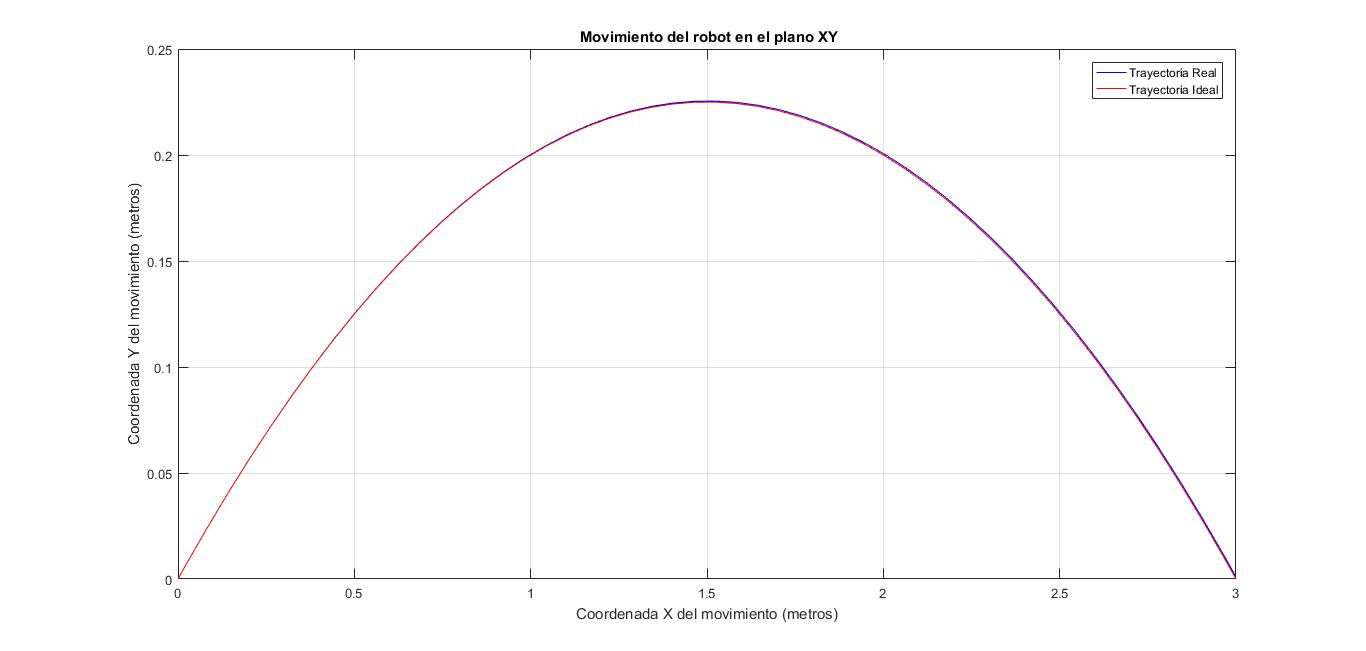
\includegraphics[width=.8\textwidth]{parab_1}
	\caption{Comparativa entre la trayectoria pedida y la obtenida}
\end{figure}


Como se puede observar, en la gráfica comparativa anterior entre la trayectoria creada por funciones y la obtenida a partir de los valores de las variables de actuación sacadas del modelo cinemático inverso, los resultados son prácticamente iguales, por lo que se puede decir que el modelo inverso es aceptable.\\

Aparte, se van a mostrar las gráficas de los valores de las variables de actuación obtenidas con la cinemática inversa, así como el valor de la variable $\varphi$:
\begin{figure}[h!]
	\centering
	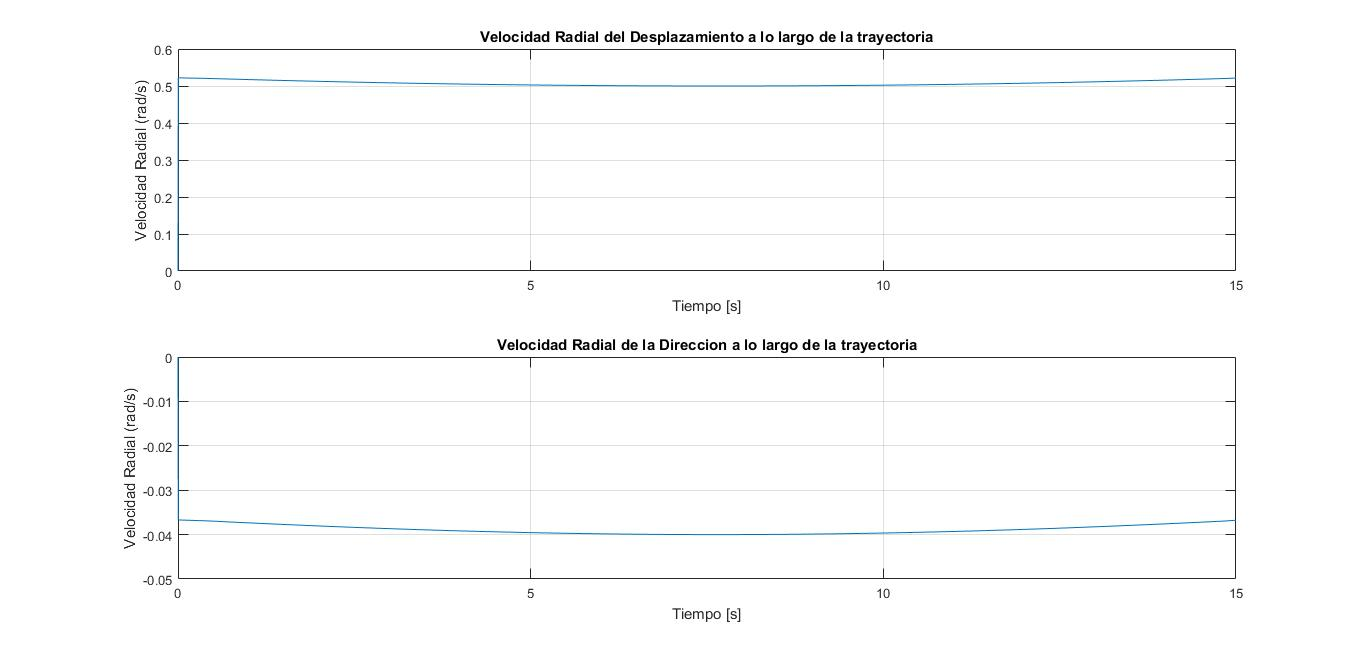
\includegraphics[width=.8\textwidth]{parab_2}
	\caption{Valores de las variables de actuación}
\end{figure}

\newpage
\begin{figure}[h!]
	\centering
	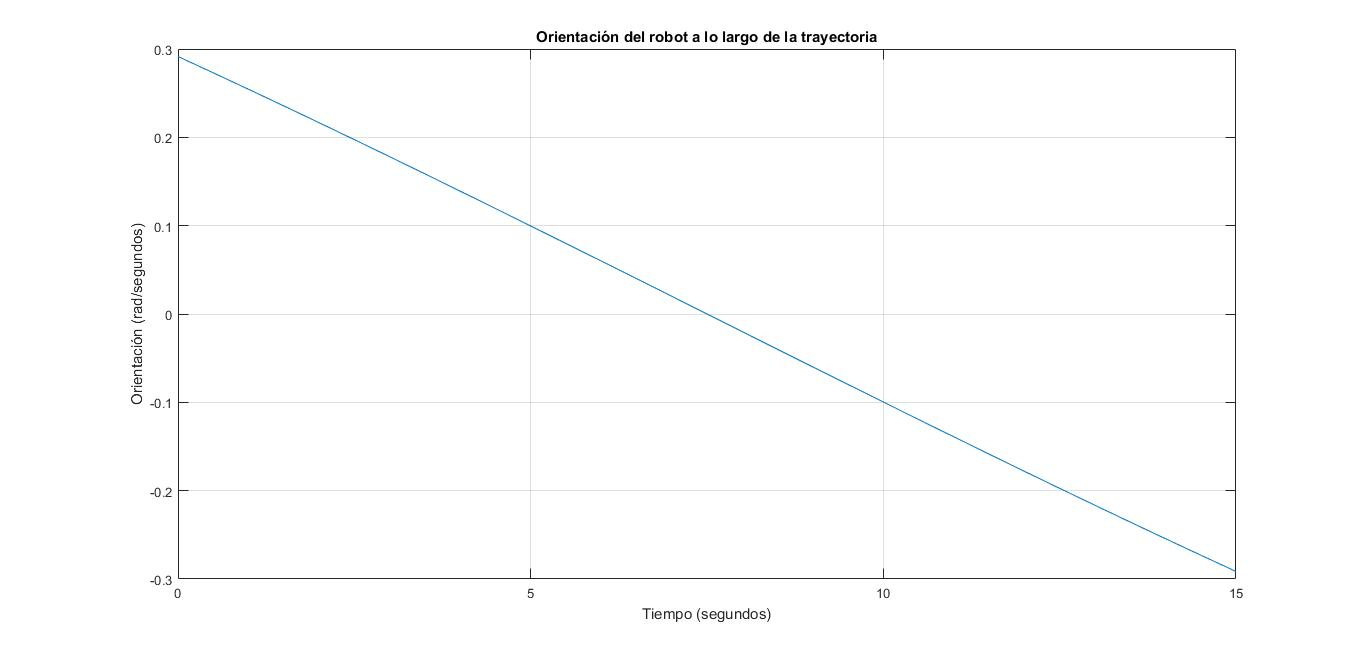
\includegraphics[width=1\textwidth]{parab_3}
	\caption{Valor de la orientación a lo largo de la trayectoria}
\end{figure}

Como se observa, en ambas velocidades no se produce saturación alguna, ya que están por debajo y por encima de sus respectivos valores de saturación. Además, con la gráfica de la orientación, se puede observar como justo a la mitad de la trayectoria, la misma es 0, ya que el robot se encuentra en paralelo al eje X en dicho momento.\\

Cabe añadir que es lo que pasaría si las variables de actuación saturasen, ya que no podrían realizar la misma trayectoria. Para ello se van a mostrar dos experimentos distintos. El primero de ellos se basa en bajar la saturación de $\dot{\theta}$ a la mitad, es decir, a $\pm$0.375:

\begin{figure}[h!]
	\centering
	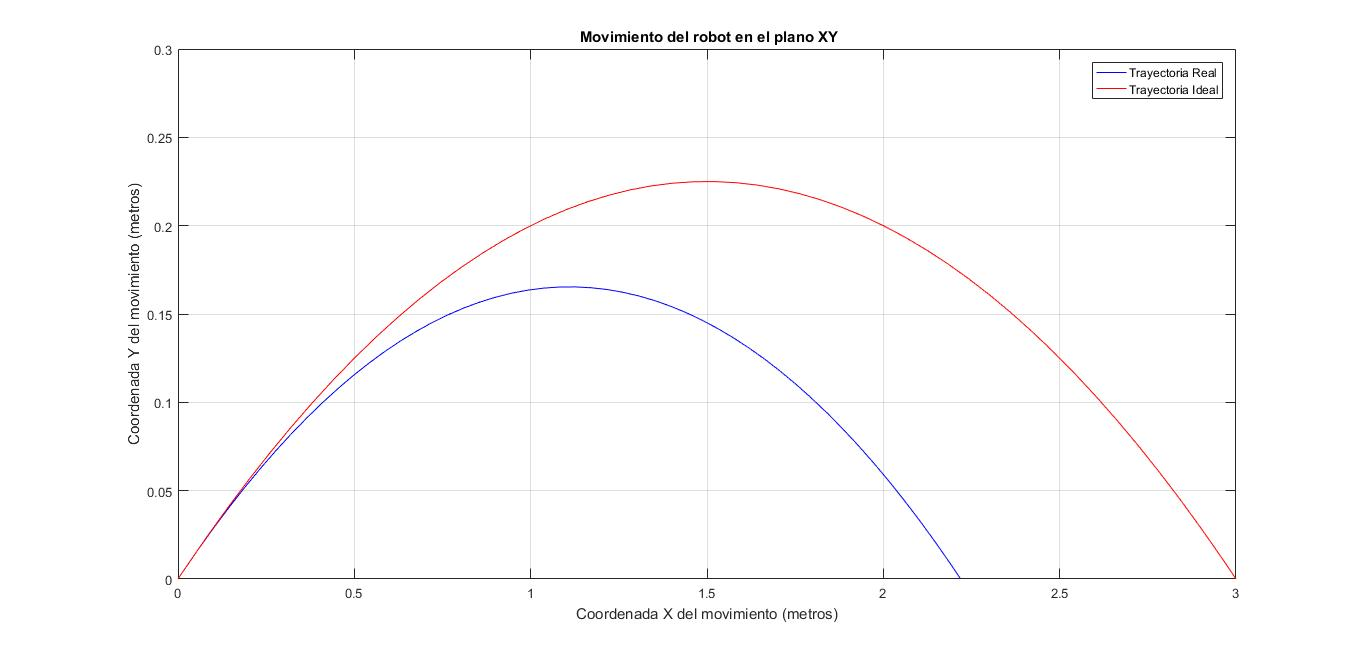
\includegraphics[width=1\textwidth]{parab_4}
	\caption{Comparativa de trayectorias con $\dot{\theta}$ saturada}
\end{figure}
\newpage
\begin{figure}[h!]
	\centering
	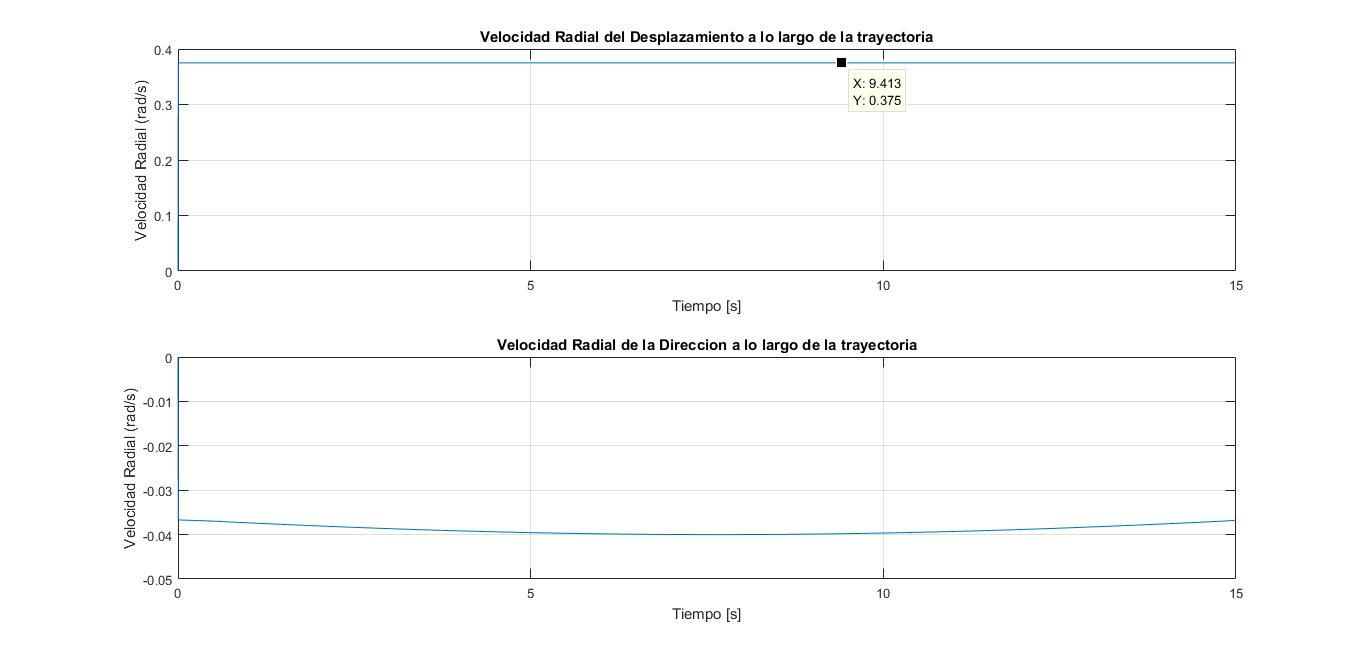
\includegraphics[width=1\textwidth]{parab_5}
	\caption{Valores de variables de actuación con saturación en $\dot{\theta}$}
\end{figure}

Como se puede observar, la trayectoria real que alcanza el robot se reduce tanto en \textit{X} como en \textit{Y}. Esto es lógico desde el punto de vista de la cinemática, puesto que al no poder alcanzar la velocidad necesaria, no llegará a ninguno de los valores objetivos en las coordenadas cartesianas. En la figura anterior se puede ver como $\dot{\theta}$ satura mientras que $\omega$ no.\\

Ahora se probará a saturar la velocidad de rotación, reduciendo el límite original a una décima parte, obteniendo una nueva saturación de $\pm$0.02618:
\begin{figure}[h!]
	\centering
	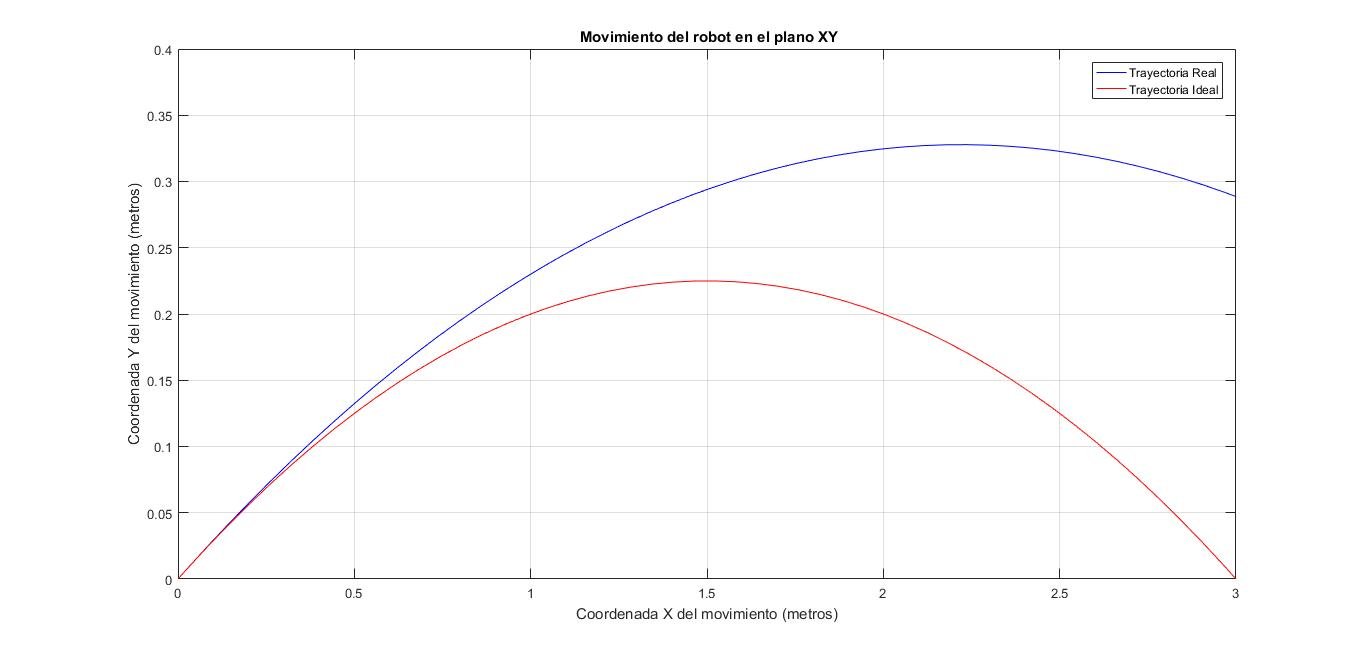
\includegraphics[width=1\textwidth]{parab_6}
	\caption{Comparativa de trayectorias con $\omega$ saturada}
\end{figure}

\newpage
\begin{figure}[h!]
	\centering
	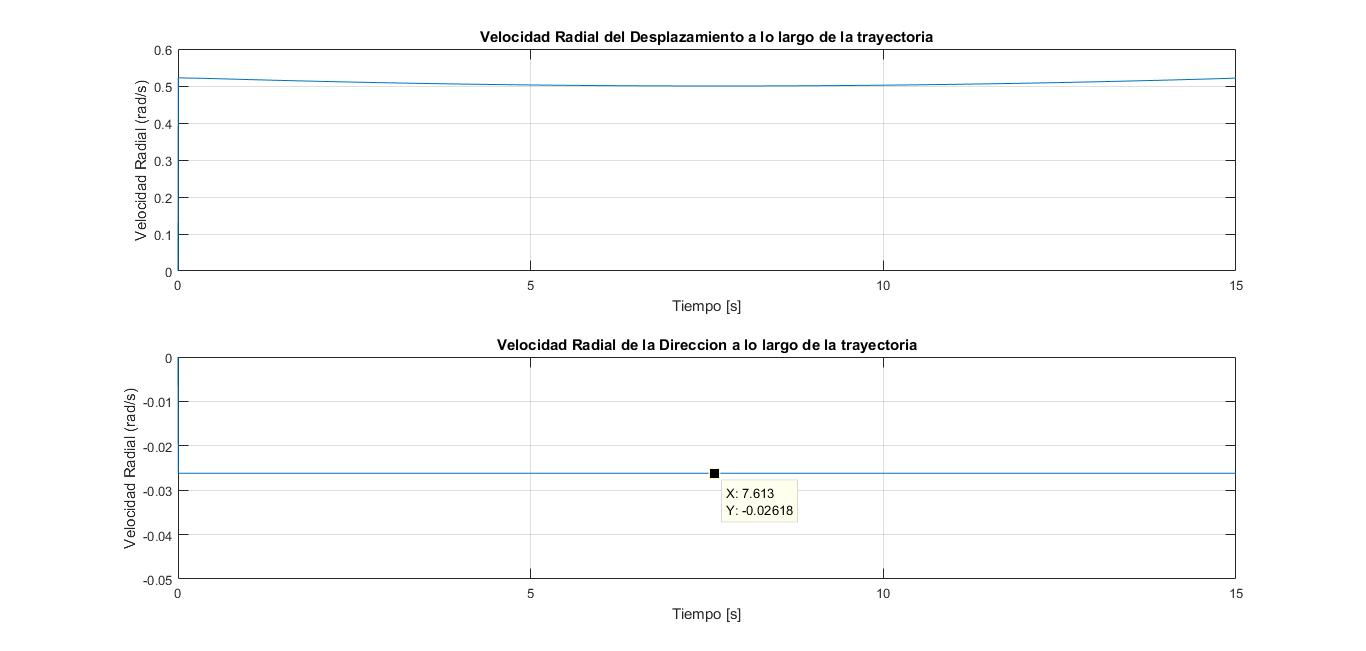
\includegraphics[width=1\textwidth]{parab_7}
	\caption{Valores de variables de actuación con saturación en $\omega$}
\end{figure}
Aquí, como también era de esperar, el robot no puede seguir la trayectoria especificada, aunque esta vez lo hace de forma distinta. Esto se debe a que tiene la velocidad de desplazamiento necesaria para alcanzar los puntos objetivos pero no la capacidad de rotar lo suficientemente rápido como para seguirlos y por ello, se sobrepasa de sus objetivos. En la figura 17 se observa la saturación en $\omega$.\\
El efecto que se produce al haber saturaciones en ambas actuaciones es una combinación de ambos resultados, es decir, el "no poder girar a tiempo" y el "no avanzar lo suficientemente rápido":
\begin{figure}[h!]
	\centering
	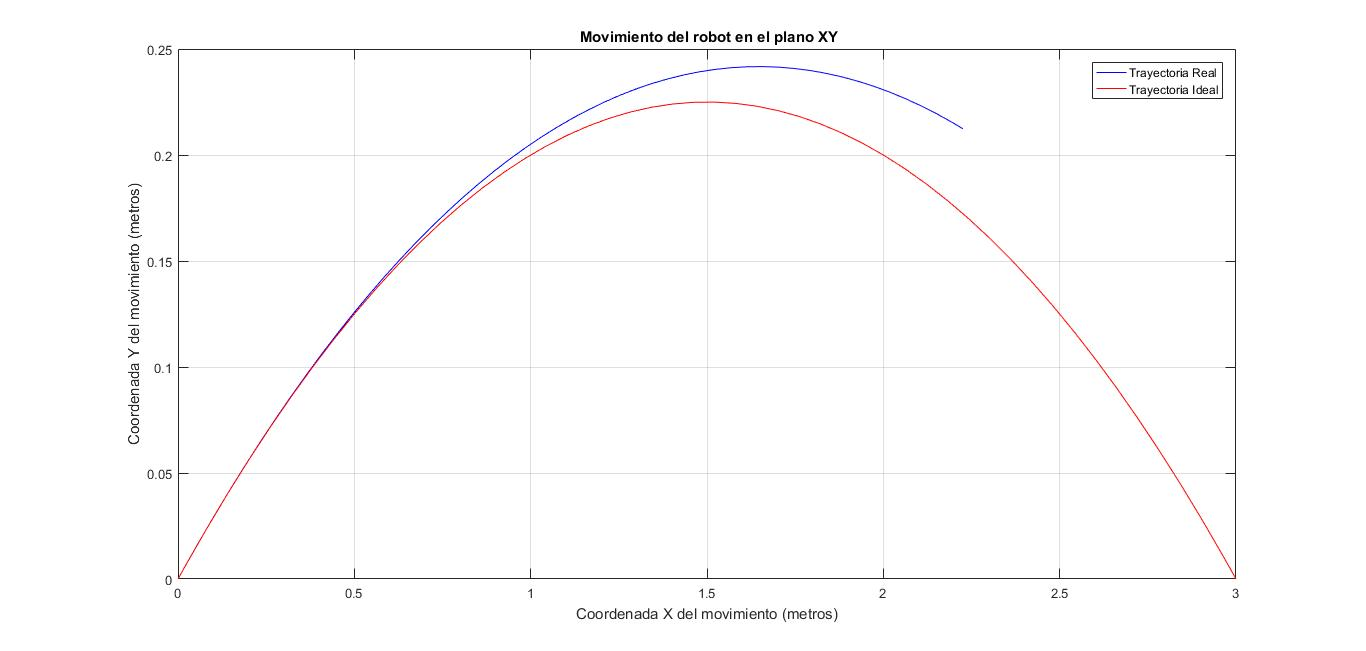
\includegraphics[width=1\textwidth]{parab_8}
	\caption{Comparativa de trayectorias con $\omega$ y $\dot{\theta}$ saturadas}
\end{figure}
\newpage
\begin{figure}[h!]
	\centering
	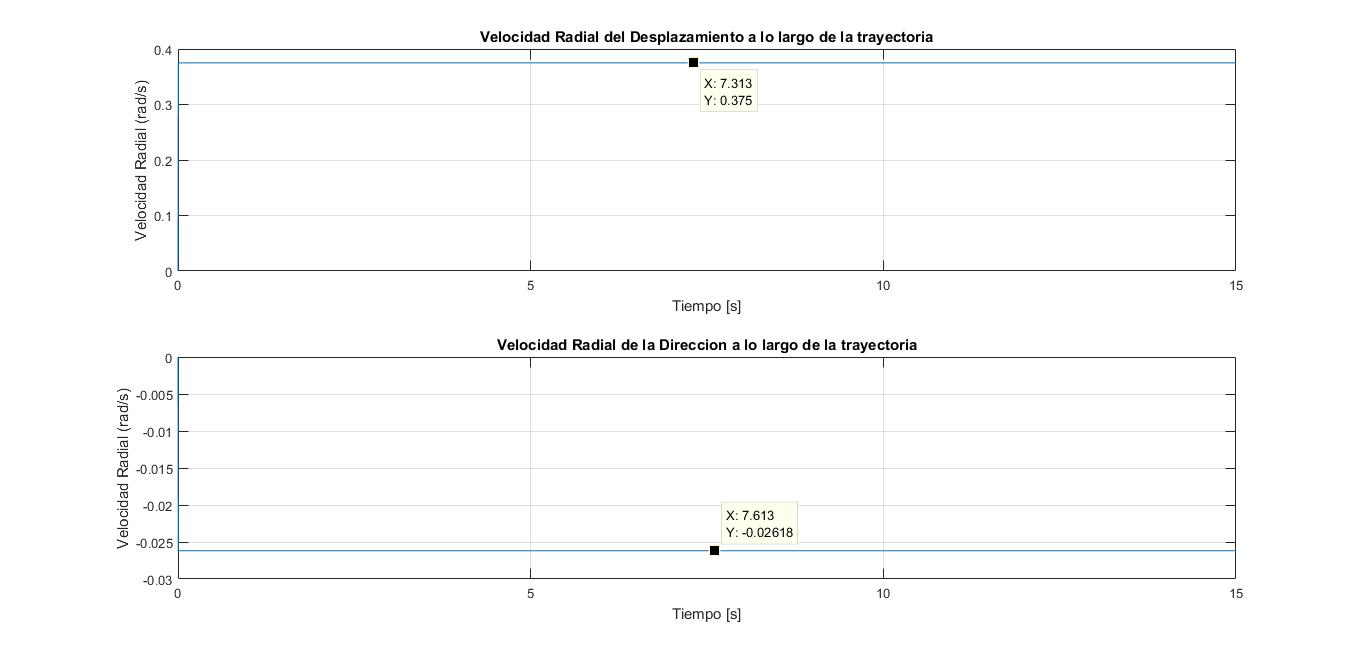
\includegraphics[width=1\textwidth]{parab_9}
	\caption{Valores de variables de actuación con saturación en $\omega$ y $\dot{\theta}$}
\end{figure}

\newpage
\section{Control dinámico}
En lo que a la implementación de un algoritmo de control dinámico sobre el robot concierne, en primer lugar será necesario complear el modelo añadiendo la dinámica de los actuadores.\\
Los actuadores del robot será supondrán 3 motores de corriente continua, cuya función de transferencia que relaciona la entrada de tensión del motor con la salida en velocidad del mismo se define del siguiente modo:
\begin{equation}
	G(s)=\frac{v(s)}{u(s)}=\frac{K}{\tau s+1}
\end{equation}
Será necesario definir el valor de la ganancia de la función de transferencia y la constante de tiempo, los cuales se obtendrán experimentalmente y unificarán toda la dinámica del motor, es decir,momento de inercia del motor, coeficiente de friccion viscosa, constante de fuerza contra-electromotriz, etcétera.
\subsection{Implementación de diversos algoritmos de control}
	\subsubsection{Control a un punto}
	\subsubsection{Control a una linea}
	\subsubsection{Control a una trayectoria}
	\subsubsection{Control a una postura}
\subsection{Ley de control \textit{Persecución pura}}

\section{Anexos y conclusiones}
\subsection{Codigos de programacion}
\subsubsection{Pruebas del modelo cinematico directo}
\lstinputlisting[caption = {caption caption caption}]{pruebasMCD.m}
\newpage
\subsubsection{Pruebas del modelo cinematico inverso}
\lstinputlisting[caption = {caption caption caption}]{pruebasMCI.m}

\end{document}
